\documentclass{article}

\usepackage[margin=0.75in, headheight=35pt, includehead, includefoot]{geometry}

\usepackage{fancyhdr}
\usepackage[T1]{fontenc}
\usepackage[shortlabels]{enumitem}
\usepackage{graphicx}
\graphicspath{ {./} }
\usepackage[export]{adjustbox}
\usepackage{booktabs}
\usepackage{forest}
\usepackage{listings}
\lstset{escapeinside={(*@}{@*)}}

\setlength{\parindent}{4em}
\setlength{\parskip}{1em}

\pagestyle{fancy}
\rhead{Alex Kitsul\\230134210\\February 25, 2021}

\begin{document}
\thispagestyle{empty}
\begin{center}
\topskip0pt
\vspace*{\fill}
\Huge Alex Kitsul\\
\Huge 230134210\\
\Huge CPSC 450\\
\Huge Assignment 4 - Report\\
\Huge February 25\\
\vspace*{\fill}
\end{center}
\pagebreak

\section*{Psedocode}
\begin{lstlisting}
main:
	number_list <- from file
	
	sorted_list, distance <- greedysort(number_list)
	Output to user sorted_list and distance
	
greedysort(number_list):
	distance = 0
	
	for i from 1 to (len(list) + 1):
		if (abs(list[i - 1]) != i):
			number_list = reversal(number_list, i)
			distance++
		if (list[i - 1] < 0):
			list[i - 1] = abs(list[i - 1])
			distance++

	return number_list, distance
			
reversal(number_list, i):
	for index, value in enumerate(number_list):
		if (abs(value) == i):
			matching_value = index
			break
			
	farther <- number_list[matching_value]
	closer <- list[i - 1]
	
	for j in range(i - 1, matching_value):
		list[j] = -list[j]
		
	return number_list
		
\end{lstlisting}

\pagebreak

\section*{Program Code}
\textbf{\underline{GreedySort.py}}
\begin{lstlisting}
def main():
    """
        Main driver method

        Parameters:

            None

        Returns:

            None. Side effect.
    """
    file_name = input("Enter file name: ")

    with open(file_name) as file:
        # Read in file
        read_string = file.read()
        # Split into usable contents
        split = read_string.split("(")[1].split(")")[0].split(" ")
        # Convert all of the values to ints
        for i in range(len(split)):
            split[i] = int(split[i])
        
        # Apply sorting
        sorted_list, reversal_distance = greedysort(split)
        print("Sorted list: ", sorted_list, "\n Distance: ", reversal_distance)
        
def greedysort(list):
    """
        Greedy Sort algorithm implementation

        Parameters:

            list (list[]): list of integer values to sort

        Returns:

            list (list[]): Sorted list
    """
    reversal_distance = 0
    # For all values in the list from 1 to the length
    for i in range(1, len(list) + 1):
        # If the absolute value of the list value is not equal to the index + 1
        if (not abs(list[i - 1]) == i):
            # Sort the list around the mismatching value
            list = reversal(list, i)
            # Increase the distance counter
            reversal_distance += 1
        # If the values after the sorting are negative (but in the right spot)
        if (list[i - 1] < 0):
            # Make the number non-negative
            list[i - 1] = abs(list[i - 1])
            # Increase the distance counter
            reversal_distance += 1

    return list, reversal_distance

def reversal(list, i):
    """
        Reversal function that takes the list, finds the next 
        breakpoint, and rotates the numbers around the breakpoint.

        Parameters:

            list (list[]): list to modify
            i (int): index value to rotate around

        Returns:

            list (list[]): List with rotated values
    """
    # Iterate through all the indexes and values in the list
    for index, value in enumerate(list):
        # If we run into a breakpoint
        if (abs(value) == i):
            # Mark the index
            matching_value = index
            break

    # Save the values in a variable so we don't lose any
    farther = list[matching_value]
    closer = list[i - 1]

    # Switch the two around
    list[i - 1] = farther
    list[matching_value] = closer

    # Invert the signs of everything between the two values
    for j in range(i - 1, matching_value):
        list[j] = -list[j]

    return list

if __name__ == "__main__":
    main()

\end{lstlisting}

\section*{Examples with Output}
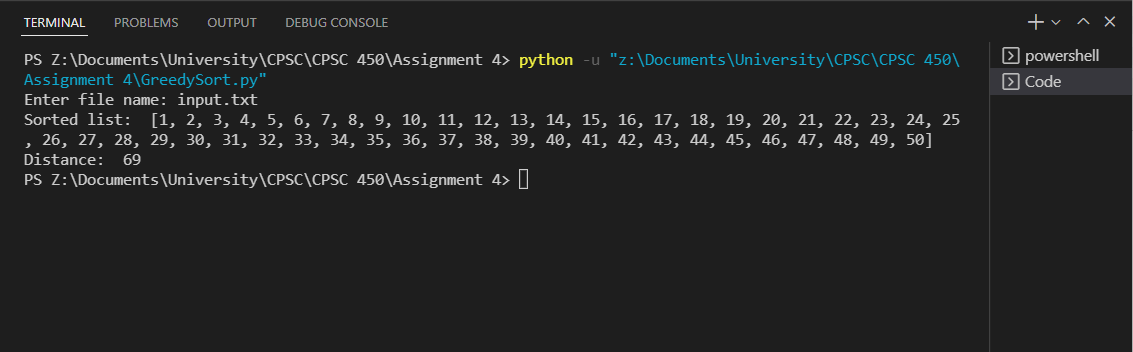
\includegraphics[scale=0.445]{ExampleInput1.png}\\

\end{document}
